\section{Spannungswandler}

\subsection{Grundlagen Bezeichnungen}
\begin{tabular}{p{250pt} p{250pt}}
D, Digitale Zahl, Wert des Datenwortes& \\
$B_0$: Bitwert 0 & LSB: Least Significant Bit\\
$B_{n-1}$: Bitwert n-1 & MSB: Most Significant Bit\\
$D = B_0\cdot 2^0 + B_1\cdot 2^1+...+B_{n-1}\cdot 2^{n-1}$&
$Vout = \frac{D}{2^n}\cdot (V_{refp}-V_{refn})+V{refn}$\\
$D = \dfrac{V_{in}-V_{refn}}{V_{refp}-V_{refn}}\cdot 2^n$
\end{tabular}

\subsection{Quantisierung}
$q = \dfrac{V_{refp}-V_{Vrefn} }{2^n}$\\

\subsection{Digitale Codes}
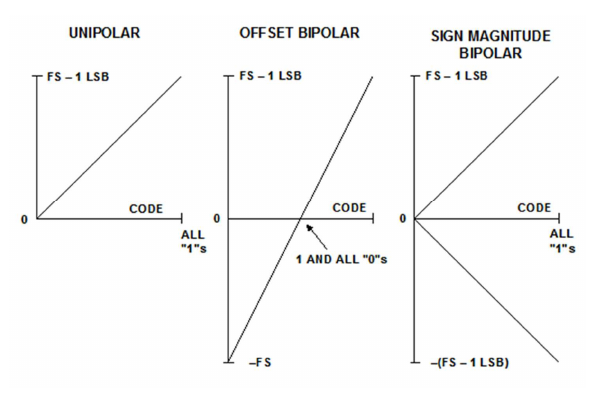
\includegraphics[width = 5cm]{images/spgwandler/01_digitalecodes}

\subsection{Ideale Wandler und Quantisierungsfehler}
Der absolute Fehler schwankt um $\pm \textonehalf$ LSB\\
$q = \dfrac{V_{refp} - V_{refn}}{2^n}$

\subsection{Signal-Rauschabstand}
PS: Leistung des Eingangssignals: $P_S = \left(\dfrac{2^{n-1}\cdot q}{\sqrt{2}}\right)^2 = 2^{2n-3}\cdot q^2$\\
PQ: Leistung des Quantisierungsrauschens unter der Annahme, dass jeder Spannungswert gleich oft vorkommt: $P_Q \approx \dfrac{q^2}{12}$\\
$SNR = 10\cdot \log(\dfrac{P_S}{P_Q}) = 10\cdot \log(1.5\cdot 2^n) = 1.76 +n\cdot 6.02 \qquad$ Pro Bit erhöht sich das SNR um 6dB. $ENOB = \dfrac{SNR_{dB}- 1.76}{6.02}$
\subsection{Abtastung}
Die Abtastung muss das Abtasttheorem von Shannon erfüllen, damit kein Aliasing entsteht.\\
%entsprechende Formeln und grafiken
Sample-Hold wirkt wie ein Tiefpassfilter, indem das Spektrum mit einer sinc-Funktion gewichtet wird.
\subsection{Kenndaten von Wandlern}
\subsubsection{Offset-Fehler}
\subsubsection{Verstärkungs-Fehler}
\subsubsection{Differentielle Nichtlinearität DNL}
\subsubsection{Kennlinien: Differentielle Nichtlinearität DNL}
\subsubsection{Integrale Nichtlinearität INL}
\subsubsection{Aperturfehler}
\subsubsection{Linearität: Spurious Free Dynamic Range SFDR}
\subsubsection{Verzögerungszeit, Settling Time}
\subsubsection{Abtast-Halteschaltung (Sample \& Hold Schaltung)}

\subsection{Digital-Analog-Wandler}
\subsubsection{Parallelverfahren}
\subsubsection{Strom-DAC}
$I_{OUT} = D\cdot I = D \cdot \dfrac{V_{REF}}{R}$
\subsubsection{Segmented String DAC}
Vorteile: viel weniger Elemente\\
Nachteile: Benötigt Buffer(offset-frei), Oder viel grössere R in Widerstandskette
\subsubsection{Wägeverfahren}

\subsubsection{Zählverfahren}
$V_{out} = \dfrac{D}{2^n}\cdot (V_{refp}-V_{refn})+V_{refn}$

\subsubsection{Kaskadierte DACs}

\subsubsection{Pipelined DACs}
